%----------------------------------------------------------------------------------------
%	PACKAGES AND THEMES
%----------------------------------------------------------------------------------------
\documentclass[aspectratio=169,xcolor=dvipsnames]{beamer}
\usetheme{SimpleDarkBlue}

\usepackage{hyperref}
\usepackage{graphicx} % Allows including images
\usepackage{booktabs} % Allows the use of \toprule, \midrule and \bottomrule in tables
\usepackage{caption}
\usepackage{subcaption}

\usepackage{listings}



%----------------------------------------------------------------------------------------
%	TITLE PAGE
%----------------------------------------------------------------------------------------

\title[short title]{Az MRC-100 műhold SZTE-s diákmoduljának szoftveres kihívásai és megoldásai} % The short title appears at the bottom of every slide, the full title is only on the title page
\subtitle{}

\author[Kiss Ádám] {Kiss Ádám}

\institute[NTU] % Your institution as it will appear on the bottom of every slide, may be shorthand to save space
{
Kiss Ádám\\
SZTE Móra Ferenc Szakkollégium\\
SZTE Elméleti Orvostudományok Doktori Iskola\\
SZTE SZAOK Élettani Intézet -- Szenzomotoros kutatólaboratórium
     % Your institution for the title page
    \vskip 3pt
}
\date{\today} % Date, can be changed to a custom date


%----------------------------------------------------------------------------------------
%	PRESENTATION SLIDES
%----------------------------------------------------------------------------------------

\begin{document}

\lstset{language=C++,
                basicstyle=\ttfamily,
                keywordstyle=\color{blue}\ttfamily,
                stringstyle=\color{red}\ttfamily,
                commentstyle=\color{green}\ttfamily,
                morecomment=[l][\color{magenta}]{\#}
}

\begin{frame}
    \titlepage
\end{frame}

\section{Bevezetés}
\begin{frame}{MRC-100}
\begin{columns}[c] 
	\column{.4\textwidth}
	\begin{figure}
		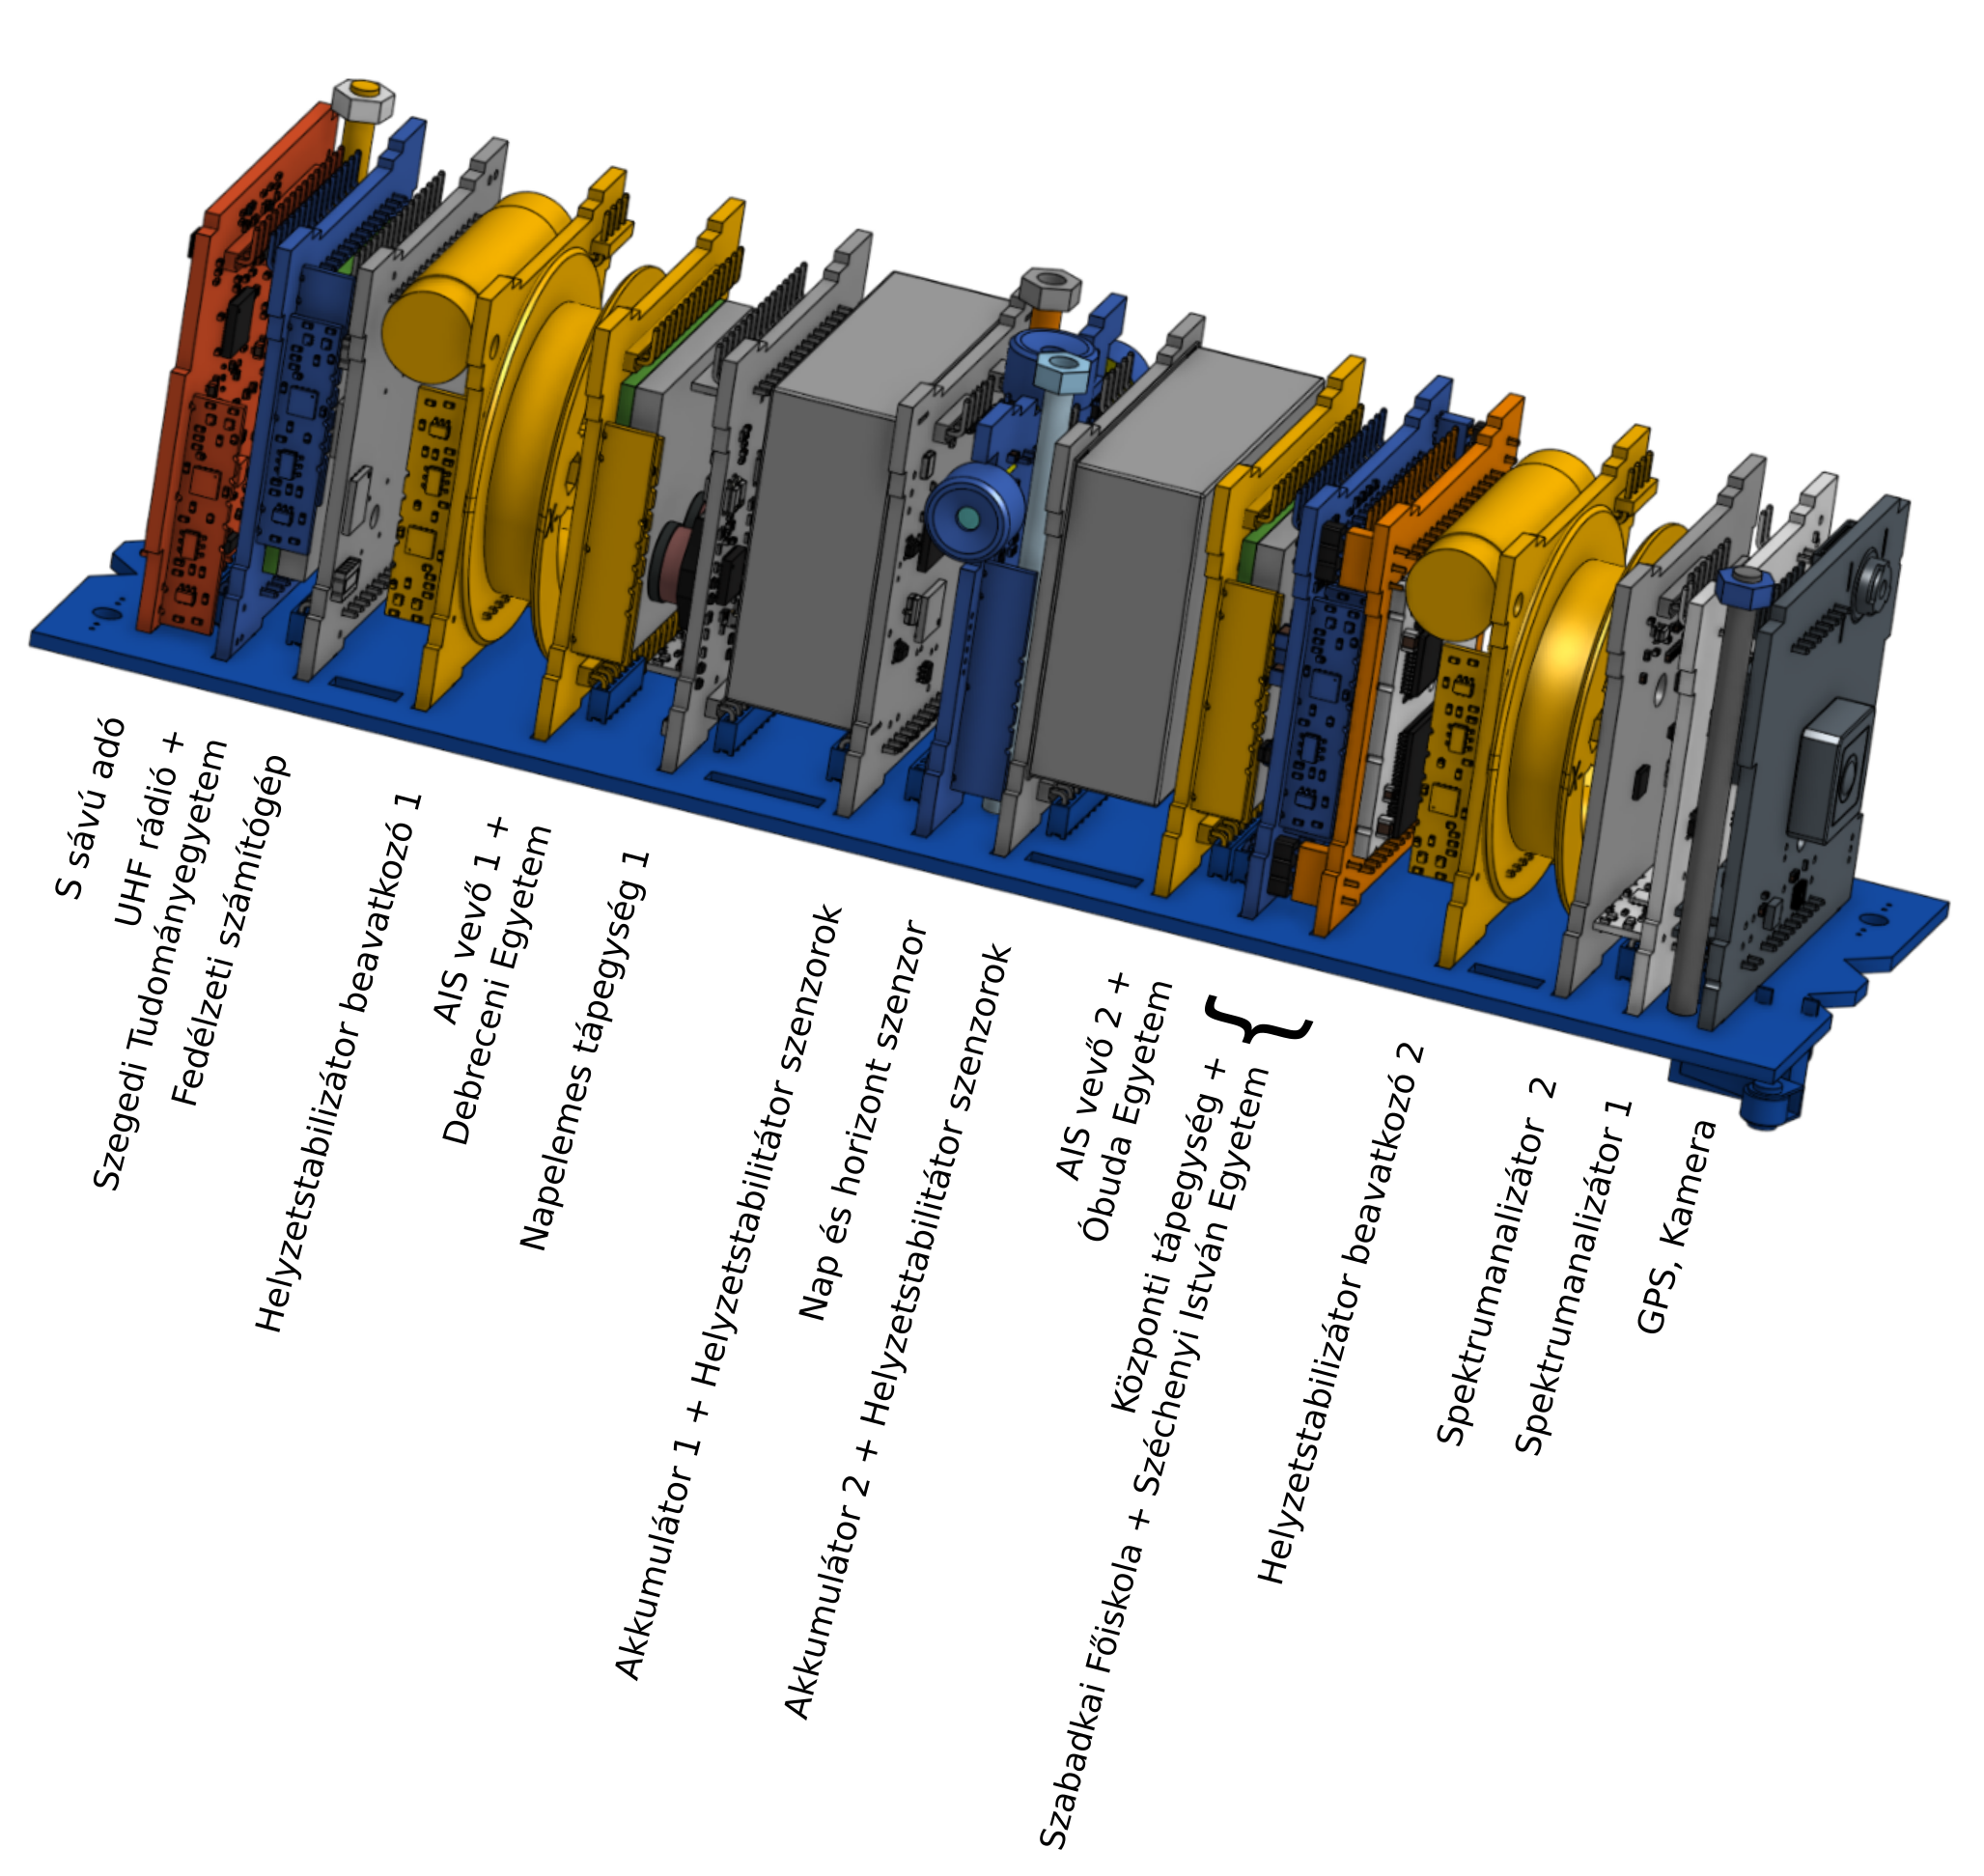
\includegraphics[width=0.95\linewidth,angle=270]{mrc100}
		\caption{Az MRC-100 műhold robbantott ábrája}
	\end{figure}
	\column{.6\textwidth} % Left column and width
	\pause
	Mi a nehezebb? Egy kicsi műholdba még kisebb modult tenni, vagy egy kicsi szoftvert egy még kisebb előadásba?
	\end{columns}
\end{frame}

\begin{frame}{Kísérleteink}
	\begin{enumerate}
		\item ADC szórás és középérték
		\item Kommunikációs busz jutter
		\item Helybéli szólások
		\item Mágneses indukció mérése
		\item Hőmérséklet mérés
		\item TicTacToe
	\end{enumerate}
\end{frame}

\begin{frame}{Hardver összegzés}
	\begin{enumerate}
		\item Vannak ADC csatornák
		\item Van egy Timer Capture bemenet
		\item UART-on kell kommunikálni adott protokollon
	\end{enumerate}
\end{frame}

\section{Szoftvertervezés}

\begin{frame}{Elvek}
	\begin{enumerate}
		\item OpenSource eszközök
		\item Overhead kerülés (erőforrásszegénység, kritikus időzítések)
		\item Átláthatóság, rendezettség, bővíthetőség
		\pause
		\item Nem probléma, ha modern szabványokat használunk
	\end{enumerate}
\end{frame}

\begin{frame}{How to STM32 free tutorial}
    \begin{columns}[c] 
        \column{.4\textwidth} % Left column and width
       		\begin{figure}[h]
				
\includegraphics[width=0.7\textwidth]{google-it}
			\end{figure}
        
        \pause

        \column{.6\textwidth} 
			\begin{enumerate}
				\item CubeIDE
				\item HAL, avagy Hardware Abstraction Layer
				\item Callback rendszer
				\item Runtime assert
			\end{enumerate}
		\end{columns}
\end{frame}

\begin{frame}{STM32 szokások}
	Ne
	\pause
	\begin{enumerate}
		\item CubeIDE $\rightarrow$ használhatatlanul lassú, sokszor hátráltat
		\pause
		\item HAL $\rightarrow$ hosszú kódra fordul, nem átlátható hibakezelés, végtelen ciklusok
		\pause
		\item Callback rendszer $\rightarrow$ bonyolult és garantáltan nem optimális időzítések
		\pause
		\item Runtime assert $\rightarrow$ fölösleges futásidejű teher, fordítás közben ismert minden
\end{enumerate}
\end{frame}

\begin{frame}{Hogyan programozzunk STM32-t?}
	\begin{enumerate}
		\item Kdevelop
		\item Regiszterírásokkal vezéreljük a konkrét hardvert
		\item Beállítjuk a gcc-t a használt utasításkészletre és regiszterkészletre \pause
		\item startup.s
		\item sysclock\_config
		\item main
		\item init függvények
	\end{enumerate}
\end{frame}

\section{Megoldásaink}

\begin{frame}[fragile]{.noinit}
	\begin{enumerate}
		\item Reboot előtt mi történt?
		\item Hányszor indult újra?
		\item Mitől lehetett az újraindulás?
	\end{enumerate}
	
	\begin{lstlisting}
	sat_stat sat_status [[gnu::section(".noinit")]];
	\end{lstlisting}
\end{frame}

\begin{frame}[fragile]{Mérések}
\begin{lstlisting}
union meas_mem_type{
    std::array<unsigned char, 1024> raw_content;
    static constexpr const std::size_t chunk_size = 12;
    static constexpr const std::size_t number_of_chunks = utils::round_up(1024, 12);

    class baud_measure_class{
        static const constexpr std::size_t histogram_width = 100;

        using histogram = std::array<uint16_t, histogram_width>;
        std::array<histogram, 5> histograms;
    public:
        void register_measure(command::Destinition dst, int16_t baud){
\end{lstlisting}
\end{frame}

\begin{frame}{Kódoljuk le}
	\begin{enumerate}
		\item Base64, char2hex... CPU idő $\leftrightarrow n+1$ keresőtábla
		\pause
		\item Compiletime string concat
		\item Compiletime GPIO init
		\item emplace
	\end{enumerate}
\end{frame}

\begin{frame}{Realitás, memóriahasználat}
Press Alt+Tab
\end{frame}

\begin{frame}{Kész! Hol hibáztam?}
	\begin{enumerate}
		\item static\_assert
		\item unit test
		\item fuzz test
		\item static code analyzer
	\end{enumerate}
\end{frame}

\begin{frame}{Hogyan kellett volna?}
	ESA kódolási szabványok
\end{frame}


\begin{frame}{Szponzoraink}

\includegraphics[width=0.2\linewidth]{fdh}

\includegraphics[width=0.2\linewidth]{ret}
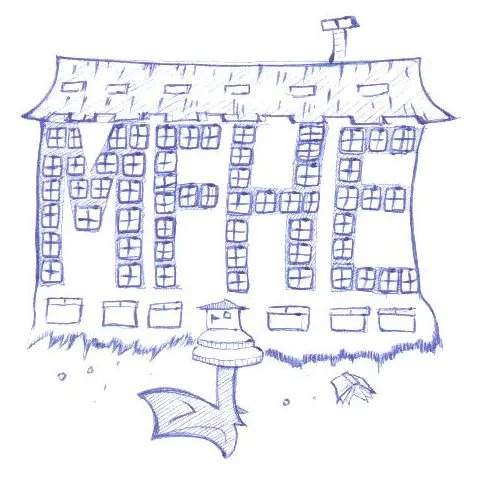
\includegraphics[width=0.2\linewidth]{mfhe}

\includegraphics[width=0.15\linewidth]{eurocircuits}

\includegraphics[width=0.2\linewidth]{csiha}
\end{frame}

\begin{frame}{Felhasznált nyílt kódú szoftverek}
	\LaTeX
	
\includegraphics[width=0.1\linewidth]{manjaro}
	
\includegraphics[width=0.1\linewidth]{linux}
	
\includegraphics[width=0.1\linewidth]{kicad}
	
\includegraphics[width=0.1\linewidth]{kdevelop}
	
\includegraphics[width=0.1\linewidth]{gcc}
	
\includegraphics[width=0.1\linewidth]{gdb}
	
\includegraphics[width=0.1\linewidth]{make}
	
\includegraphics[width=0.1\linewidth]{vim}
	
\includegraphics[width=0.1\linewidth]{llvm}
	
\includegraphics[width=0.1\linewidth]{bash}
	
\includegraphics[width=0.1\linewidth]{git}
	
\includegraphics[width=0.1\linewidth]{kde}
	
\includegraphics[width=0.1\linewidth]{gnome}
\end{frame}


\begin{frame}{További köszönet}
	Akik nélkül nem jöhetett volna össze: Antal Levente, Kiszel Pál, Kovács Adrienn, Oltvári Zsófia, Südi Tamás, Szabó Andrea, Szendefi Dániel, Tokai Eszter.
	Köszönöm a közös munkát, a közös élményt és támogatást!
	\vspace{1cm}
	\par Köszönöm az SZTE Móra Ferenc Szakkollégiumnak, hogy befogadta a projektet! Külön köszönet Kovács Attila igazgató úrnak.
	\vspace{1cm} \par Köszönet a BME-nek a lehetőségért. Nélkülük ez el se indulhatott volna. Külön köszönet Gschwindt Andrásnak.
\end{frame}

\begin{frame}
    \Huge{\centerline{Köszönöm a figyelmet!}}
\end{frame}

\end{document}
